\documentclass{article}
\title{Atreus Keyboard Assembly}
\date{ }
\usepackage{graphicx}
\usepackage{geometry}
\usepackage{wrapfig}
\newgeometry{margin=3cm}
\begin{document}
\setlength{\parindent}{0cm}
\maketitle
\section{Prerequisites}

In order to assemble your keyboard, you'll need your kit plus a few
other tools. The kit should contain these parts and a few spares:

\begin{itemize}
\item Case (top plate, switch plate, spacer, bottom plate)
\item Sandpaper
\item Finishing wax (mixture of beeswax and mineral oil)
\item Diodes (42)
\item Key switches (37 tactile or clicky, 5 red)
\item A-Star Micro controller
\item Printed circuit board (PCB)
\item Machine screws and nuts (8 each, 16mm M3 size)
\item Key caps (40 normal, 2 long)
\item USB micro cable
\item Rubber feet
\end{itemize}

You'll also need to have these on hand:

\begin{itemize}
\item Brush for applying finishing wax (a toothbrush will do)
\item Soldering iron and solder (thin solder and an iron with a sharp tip)
\item Wire cutters
\item Rags or paper towels to lay the parts down on during construction
\end{itemize}

\vspace{1em}

The latest version of this document can always be found
online.\footnote{http://atreus.technomancy.us/assembly.pdf} If you're
reading a black-and-white printed copy, you may find some of the
photos clearer in color onscreen. This copy describes the
circuit-board-based kit. If you are hand-wiring a board, see the older
assembly
guide.\footnote{http://atreus.technomancy.us/assembly-hand-wired.pdf}
The photos in this guide depict Matias switches, (with rectangular
switch stems) but you can use Cherry MX switches (with stems shaped
like a +) as well. The assembly steps are the same in either case.

\section{Sanding}

Start by sanding down both sides of each piece. You may want to
hold two pieces together while sanding for strength or placing it on a
flat surface you don't mind scruffing up; too much pressure on a
single plate could damage it.

\vspace{1em}
\noindent\makebox[\textwidth]{%
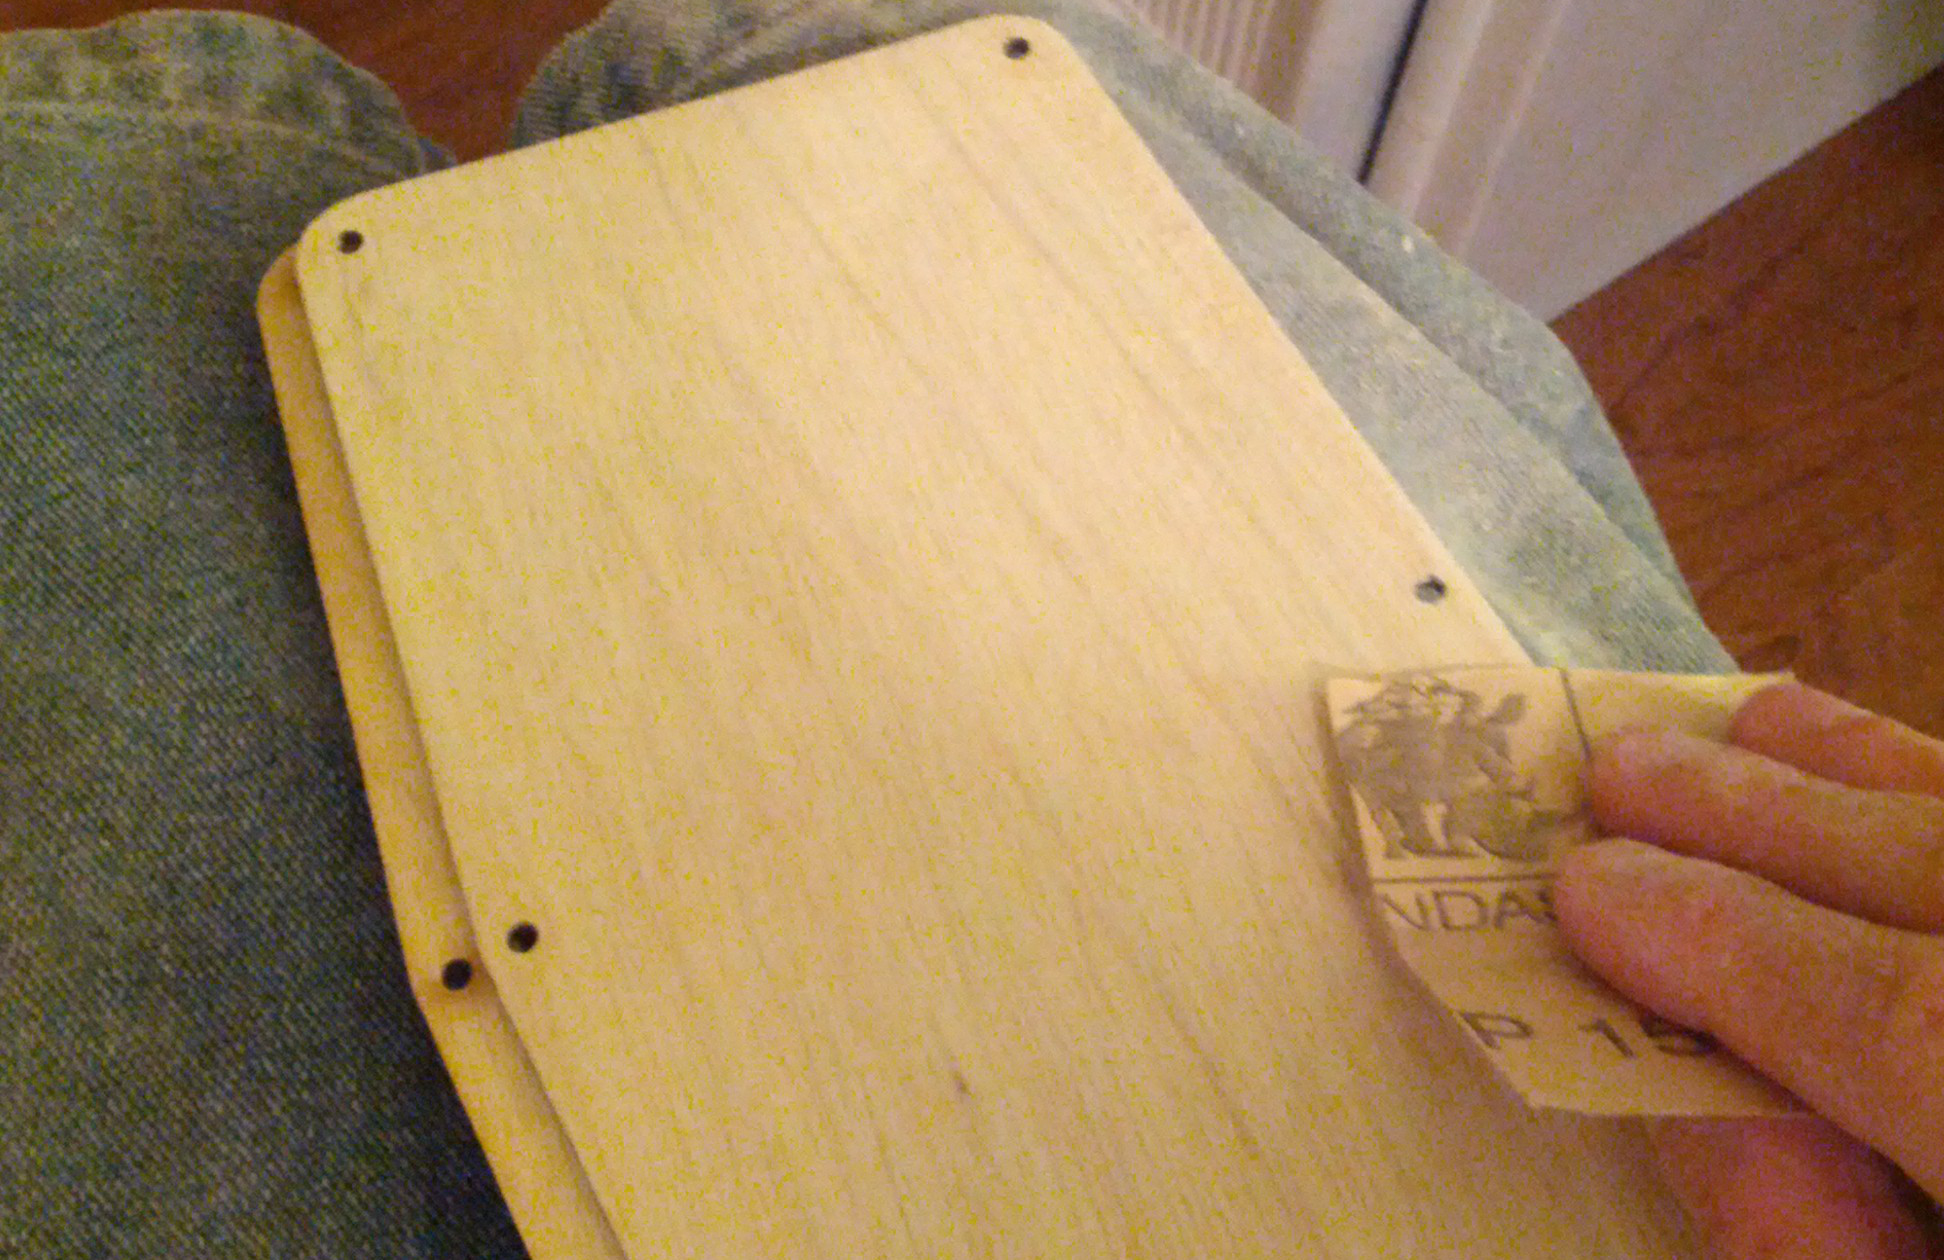
\includegraphics[width=0.7\linewidth]{sanding.jpg}}
\vspace{1em}

Keep in mind that the top side of the top plate and the bottom side of
the bottom plate are the only surfaces that are exposed to the touch
once the keyboard is fully assembled, so these will need the most
attention when sanding. You can sand the other surfaces as well just
to get the scorch marks off, but you don't need to worry about how
smooth the inner surfaces feel to the touch. Be sure to get all the
wood dust off the pieces before you go on. A clean tack cloth or other
fine cloth works well.

\section{Finishing}

%% TODO: mention polyurethane

You have two options when it comes to finishing. The easiest way is to
proceed with the wax/oil mixture included in the kit. The other option
is to apply several layers of lacquer and wet sand it down in
between coats. This requires buying more supplies and takes significantly
longer, but it results in a sturdier, shinier
finish.\footnote{http://atreus.technomancy.us/lacquer.gif} The steps
for the lacquered finish are described in a separate
document,\footnote{http://atreus.technomancy.us/lacquer.pdf} and the
rest of this section describes the quicker finishing method.

\vspace{1em}

Some people don't like the look of the exposed edges charred from the
laser cutter. You can choose to sand off the charring, or alternately
cover it all with black ink from a sharpie for a more consistent look.

\vspace{1em}

Open up the wax/oil mixture. Apply some to the brush and start
spreading it over one side of each case piece. The color of the wood
will darken as it absorbs the oil. Try to ensure it's spread
evenly. Be more generous with the oil on the outer exposed
surfaces. Once you've spread it with the brush, you can use your
fingers to work the wax into the wood more deeply. If you need to
reapply the finishing in the future, butcher block conditioner is
readily available in stores and will do the job nicely.

\vspace{1em}
\noindent\makebox[\textwidth]{%
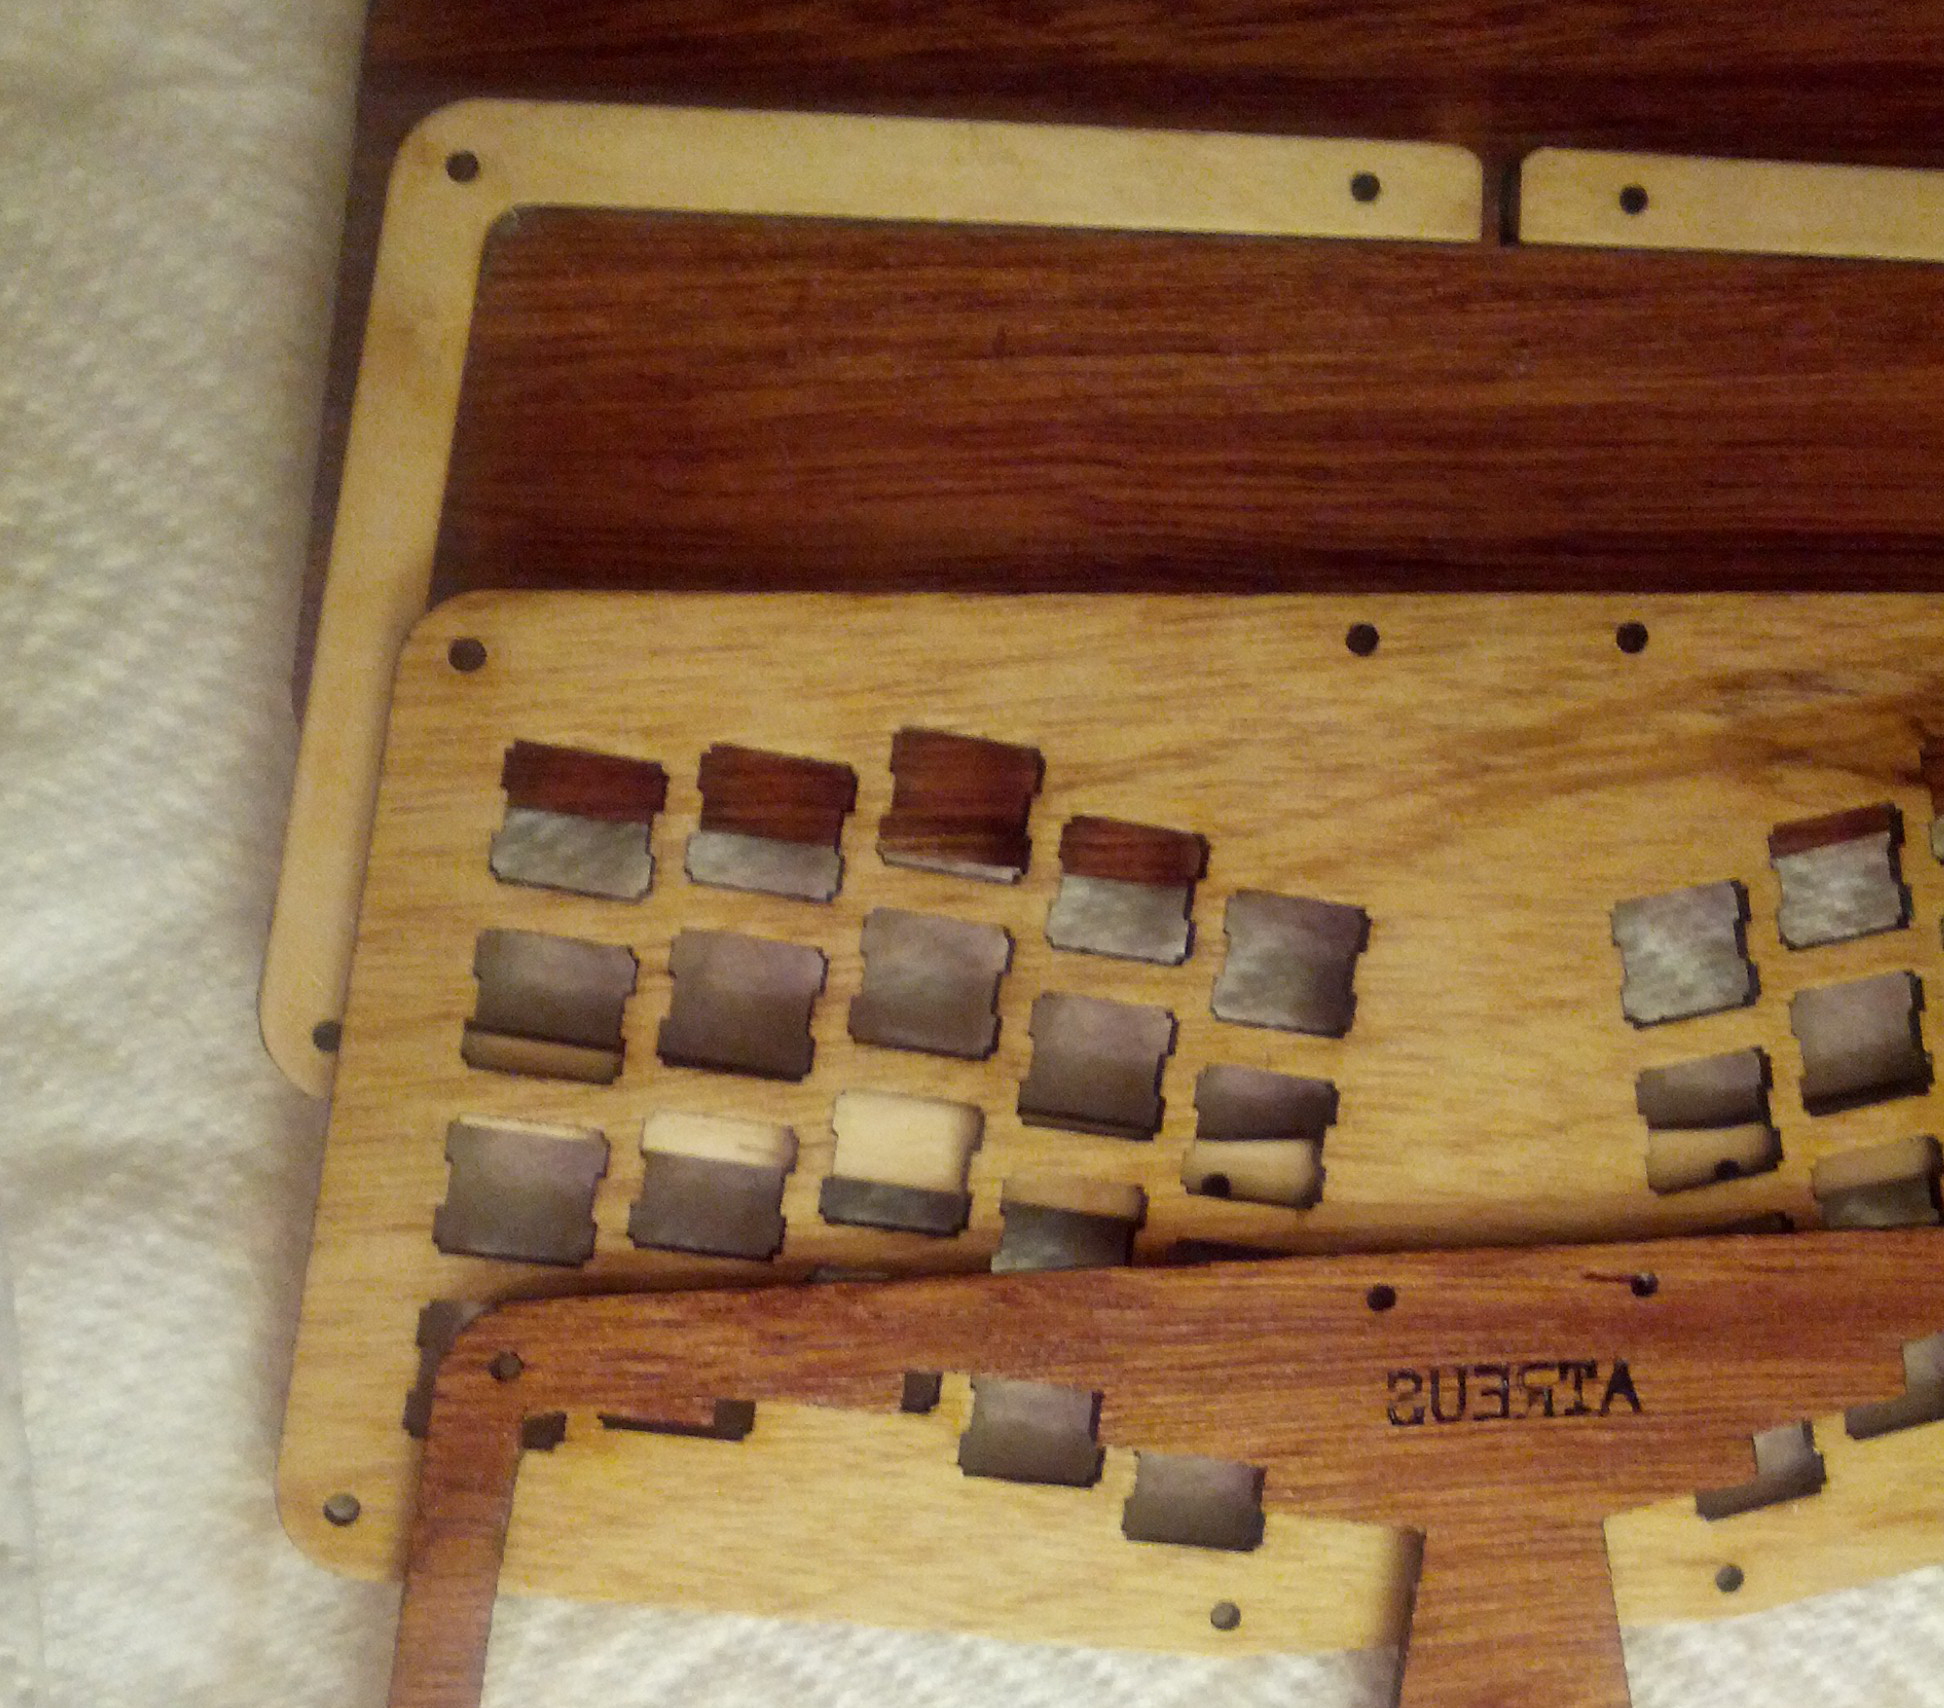
\includegraphics[width=0.7\linewidth]{oiled.jpg}}
\vspace{1em}

As your brush goes over the edges of the laser-cut wood, it will get
dirty from charred wood particles. After you've finished oiling one
side of each piece, it's best to wash out the brush. Be sure it's
fully dry before going on.

\section{Drying}

Once one side of each piece is finished, you'll need to lay them out
for a half hour or so to let them dry. (Longer if using lacquer.) Once
one side is dry, repeat the process on the other side. After you've
finished the construction you can come back and add another few coats
to the outermost surfaces for a smoother texture. Once it's dried for
a while, wipe the excess off. While you're waiting, you can start
soldering the diodes and controller onto the circuit board, but don't
solder any switches in before the switch plate is ready or you'll just
need to remove them later.

\section{Diodes}

If you've never soldered before, there are plenty of good
introductions online.\footnote{This one from Adafruit is great:
  https://learn.adafruit.com/adafruit-guide-excellent-soldering/tools}
Coat the tip of the hot iron thinly with some solder before you
start. The key is to use the iron to heat both parts of the joint for
a second or two, then bring in a dab of the solder and let it melt and
stick to the component and the circuit board pad.

\vspace{1em}

Take five diodes at a time and bend them into a U shape. Place them
into the diode holes next to each switch slot on the unlabeled side of
the board. Each diode has a black band on it; the band should be
pointing in the direction of the arrow on the printed side of the
board. Once all five are in, pinch the legs of the diodes together to
keep them from falling out, then flip the board over and solder them
in place. Make sure they don't protrude off the board more than necessary.

\vspace{1em}
\noindent\makebox[\textwidth]{%
  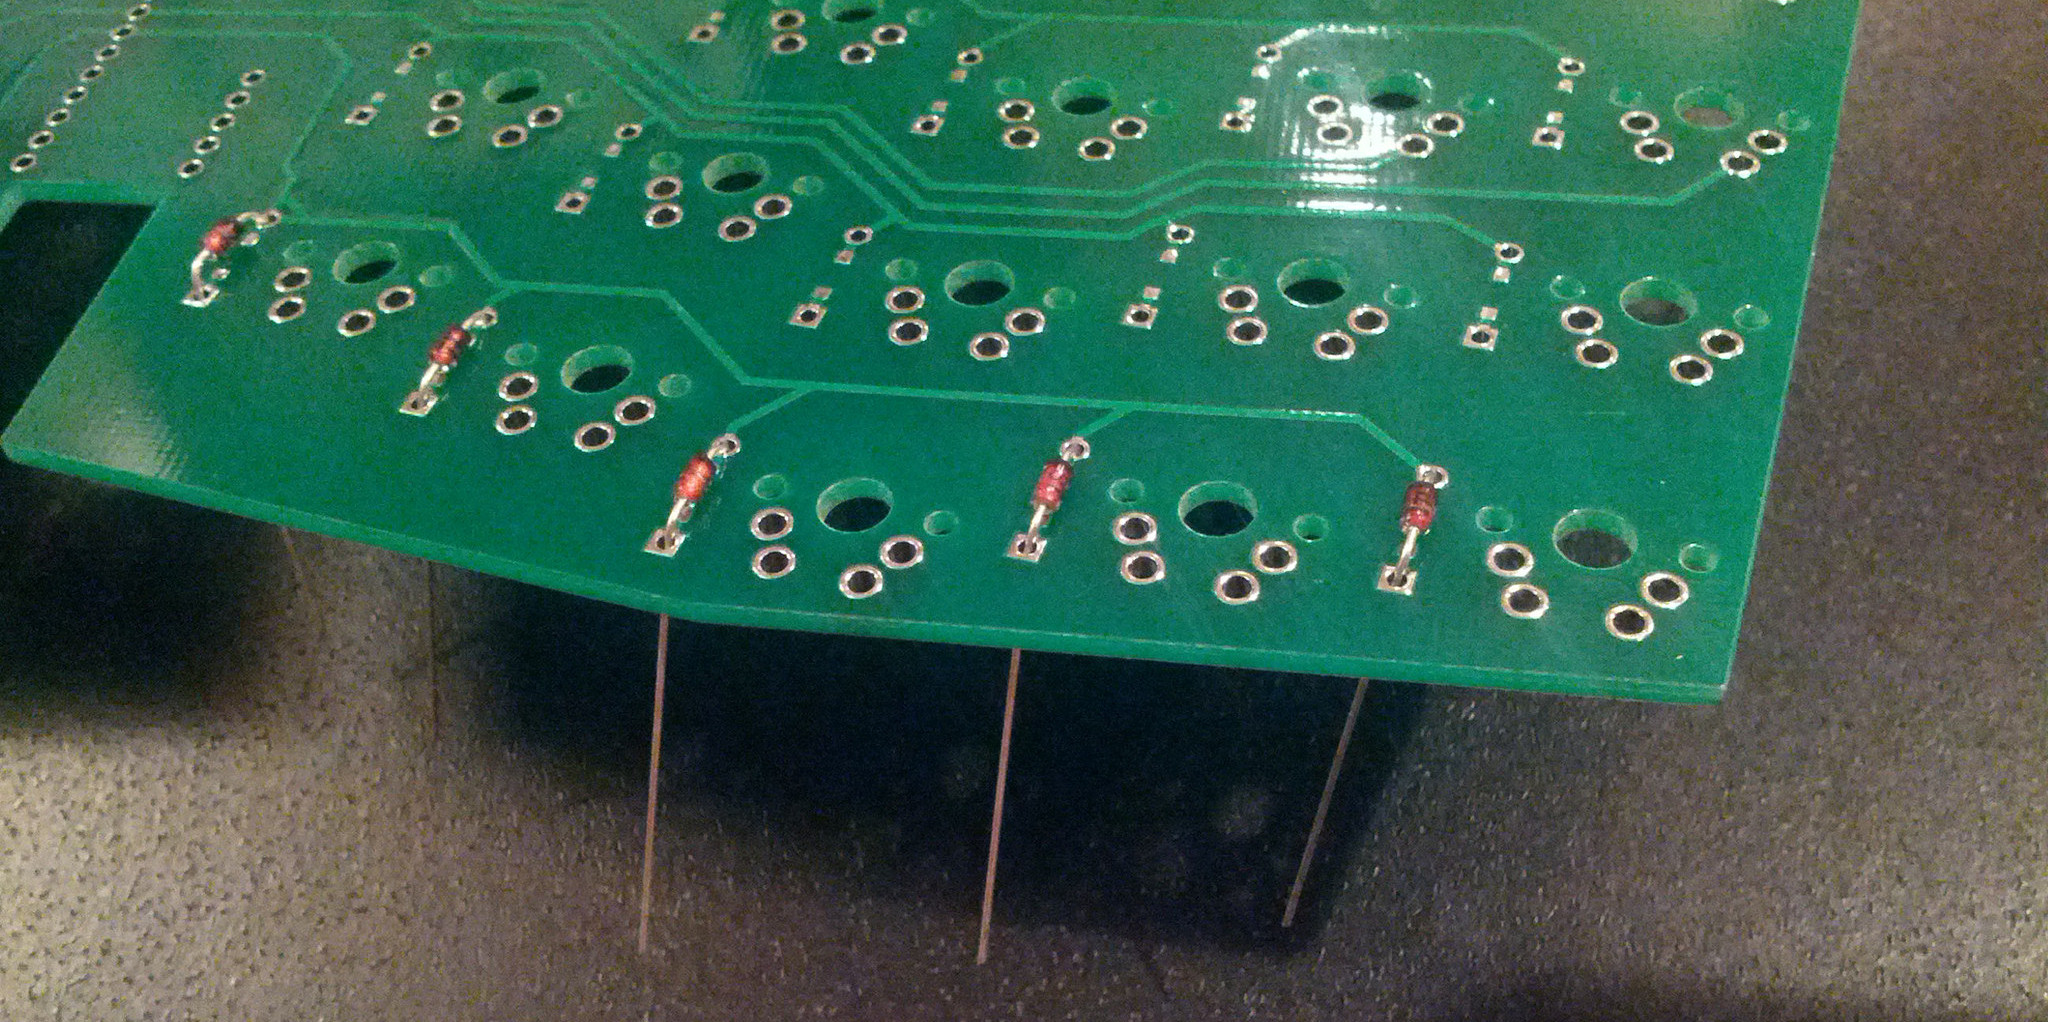
\includegraphics[width=0.7\linewidth]{diodes.jpg}}
\vspace{1em}

In the photo the diodes are inserted from the back of the circuit
board, but it will work just as well to insert them from the front as
long as the black band is oriented correctly. Once they're soldered,
trim the diode legs with wire cutters. Grip the diode leg as you
trim it to keep it from flying across the room. Keep the diode legs;
they will be needed in the next step. Repeat until each diode position
is filled.

\section{Controller}

Once the diodes are in place, you can begin attaching the controller.
If the controller came in a pink bag with its own header pins, you may
be tempted to use them to connect the controller to the circuit
board. Don't do this--they are too big and will prevent the case from
closing when you're done. We will be using the diode legs we just
trimmed instead.

\vspace{1em}

First take the PCB with the labeled side down and fill the four corner
holes in the center ``A-STAR'' section with solder. Insert diode legs
into these holes while melting the solder. Then repeat the process for
the other holes on the left, keeping them pointing as straight as possible.

\vspace{1em}
\noindent\makebox[\textwidth]{%
  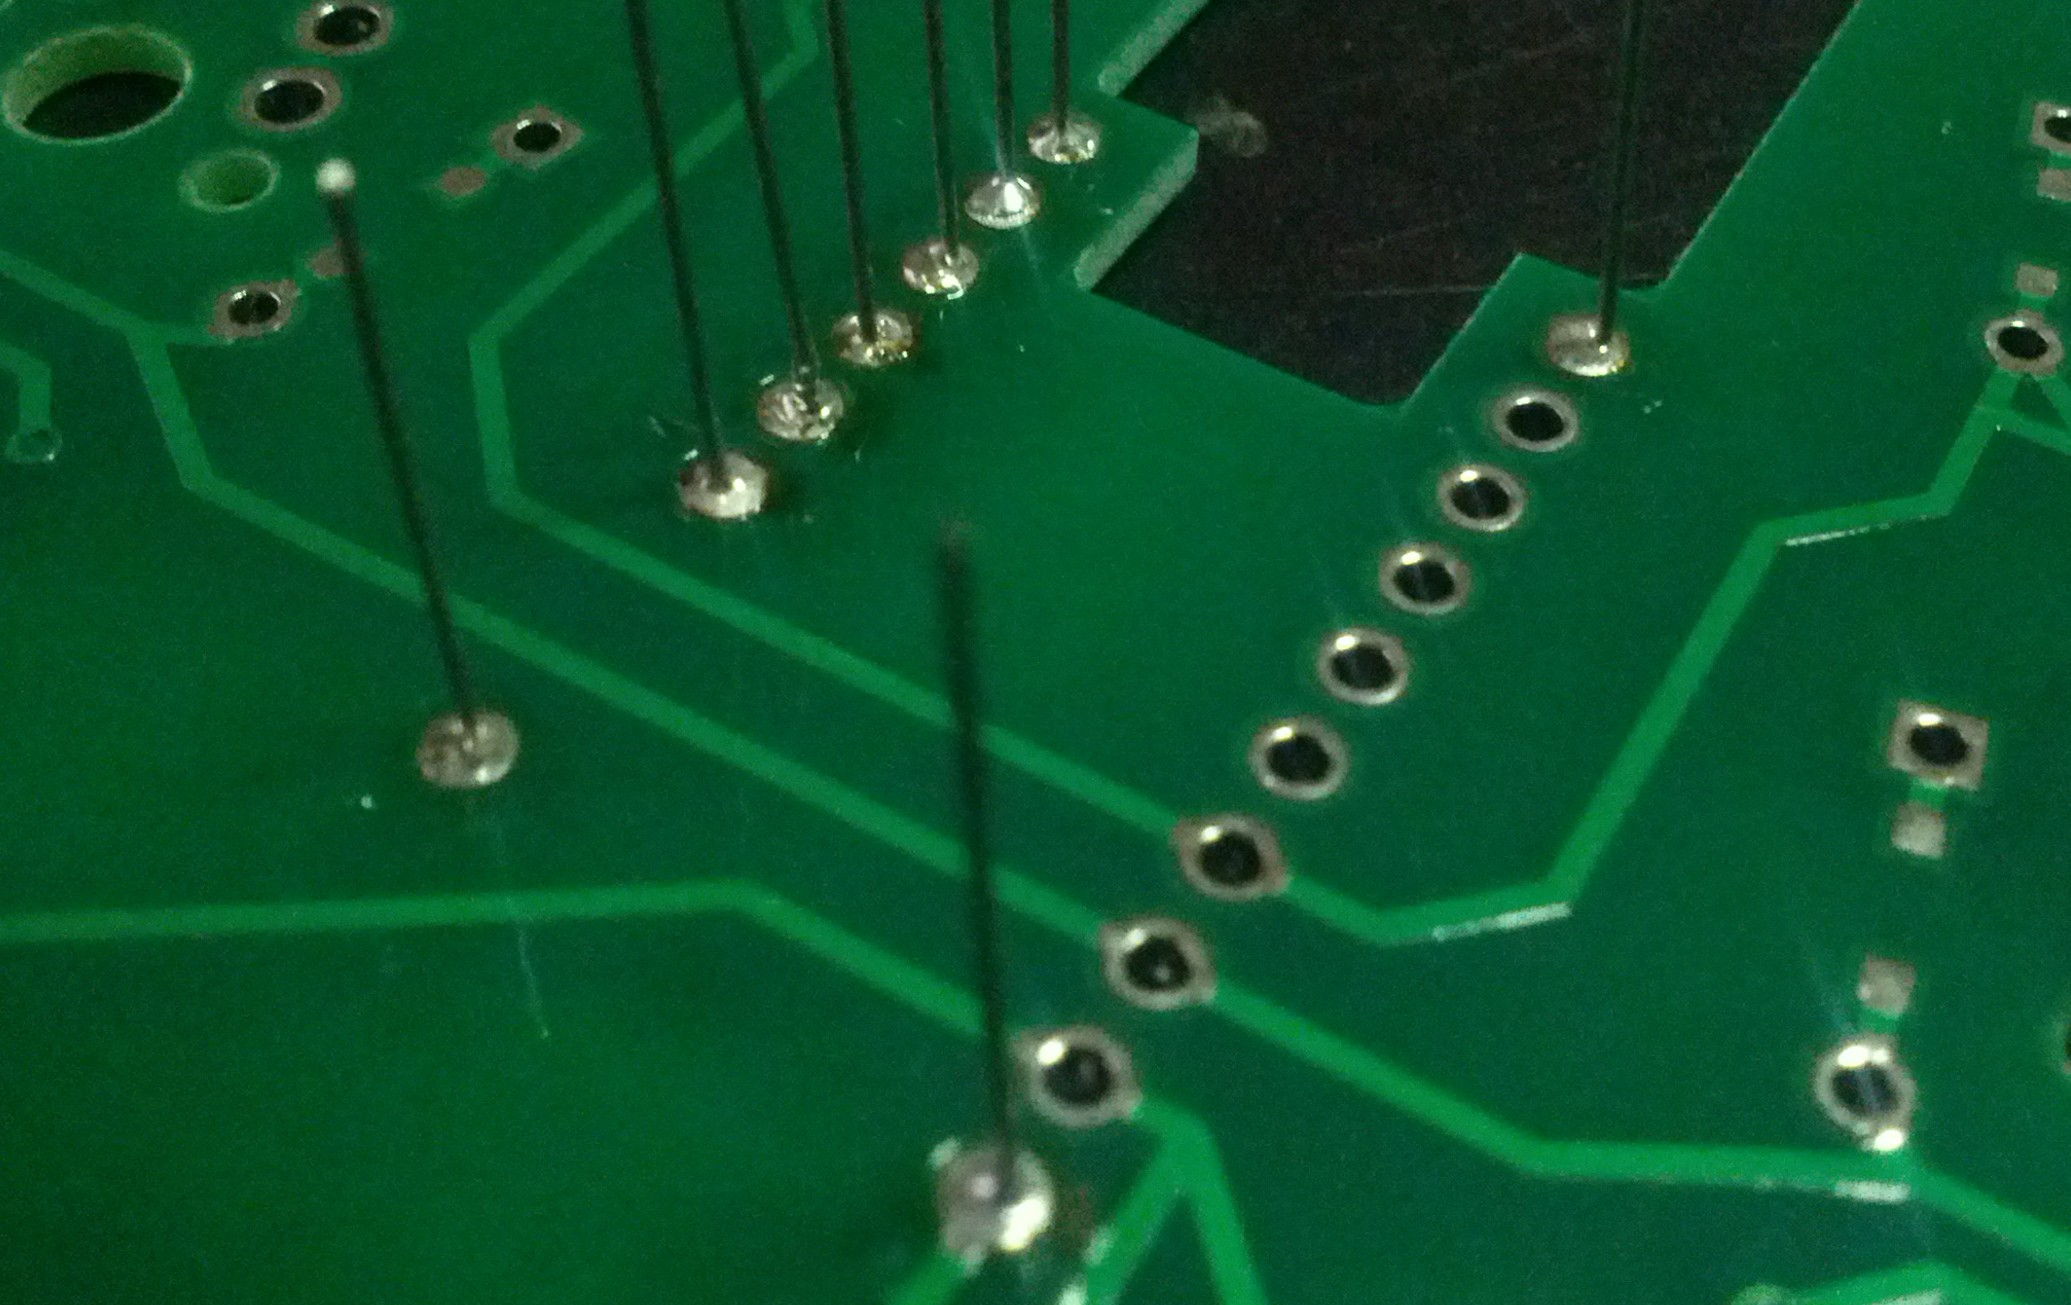
\includegraphics[width=0.8\linewidth]{many-pins.jpg}}
\vspace{1em}

Fit the controller over the pins you've attached so far. Solder the
four corner pins already connected to the PCB into the corners of the
controller. (The bottom left corner is unused; the pin above is used
instead.) Try to ensure the controller is as close to the PCB as
possible and not at an angle. Then solder the other left-side diode
legs into the controller as well. Trim them all with your wire
cutters when they are secure.

\vspace{1em}

Eight right-side holes remain. For these, bend four diode legs at a
time into an L shape, and insert them into four of the remaining
holes. Flip the board over and solder the protruding diode legs to the
PCB, then trim them down and flip the board back over. Straighten the
diode legs, then solder and trim them. Repeat for the remaining
unpopulated holes. From the PCB side, all the holes will be used, but
from the controller side, there will be some unused.

\vspace{1em}
\noindent\makebox[\textwidth]{%
  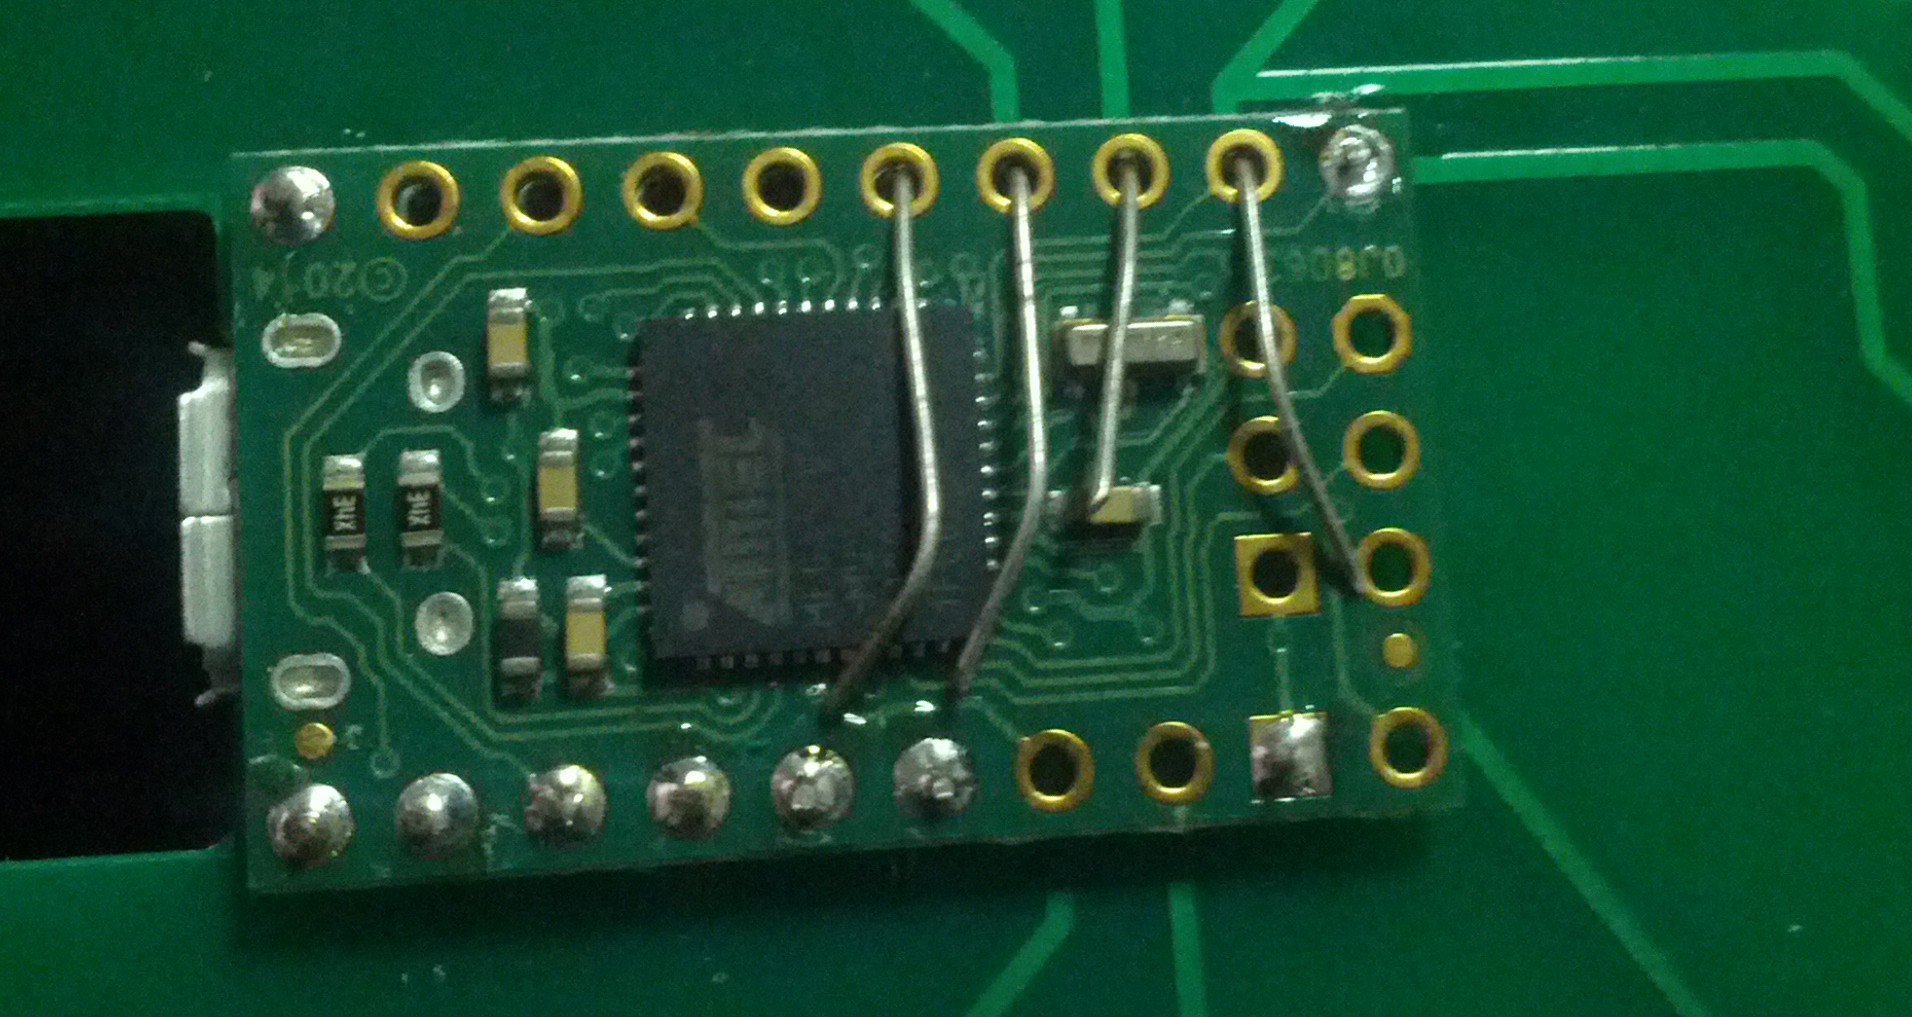
\includegraphics[width=0.8\linewidth]{bent-legs.jpg}}
\vspace{1em}

Before you go on, take the time to double-check the solder joints on
the controller. The solder should fill the hole completely without
spilling over to adjacent holes, and the legs should be secure. Also
check that all the diodes are facing the correct direction with the
black band pointing to the bottom of the board.

\section{Firmware}

Installing the firmware now isn't strictly necessary, but it will
allow you to spot mistakes before the board is finished.

\vspace{1em}

\begin{wrapfigure}{r}{0.25\linewidth}
  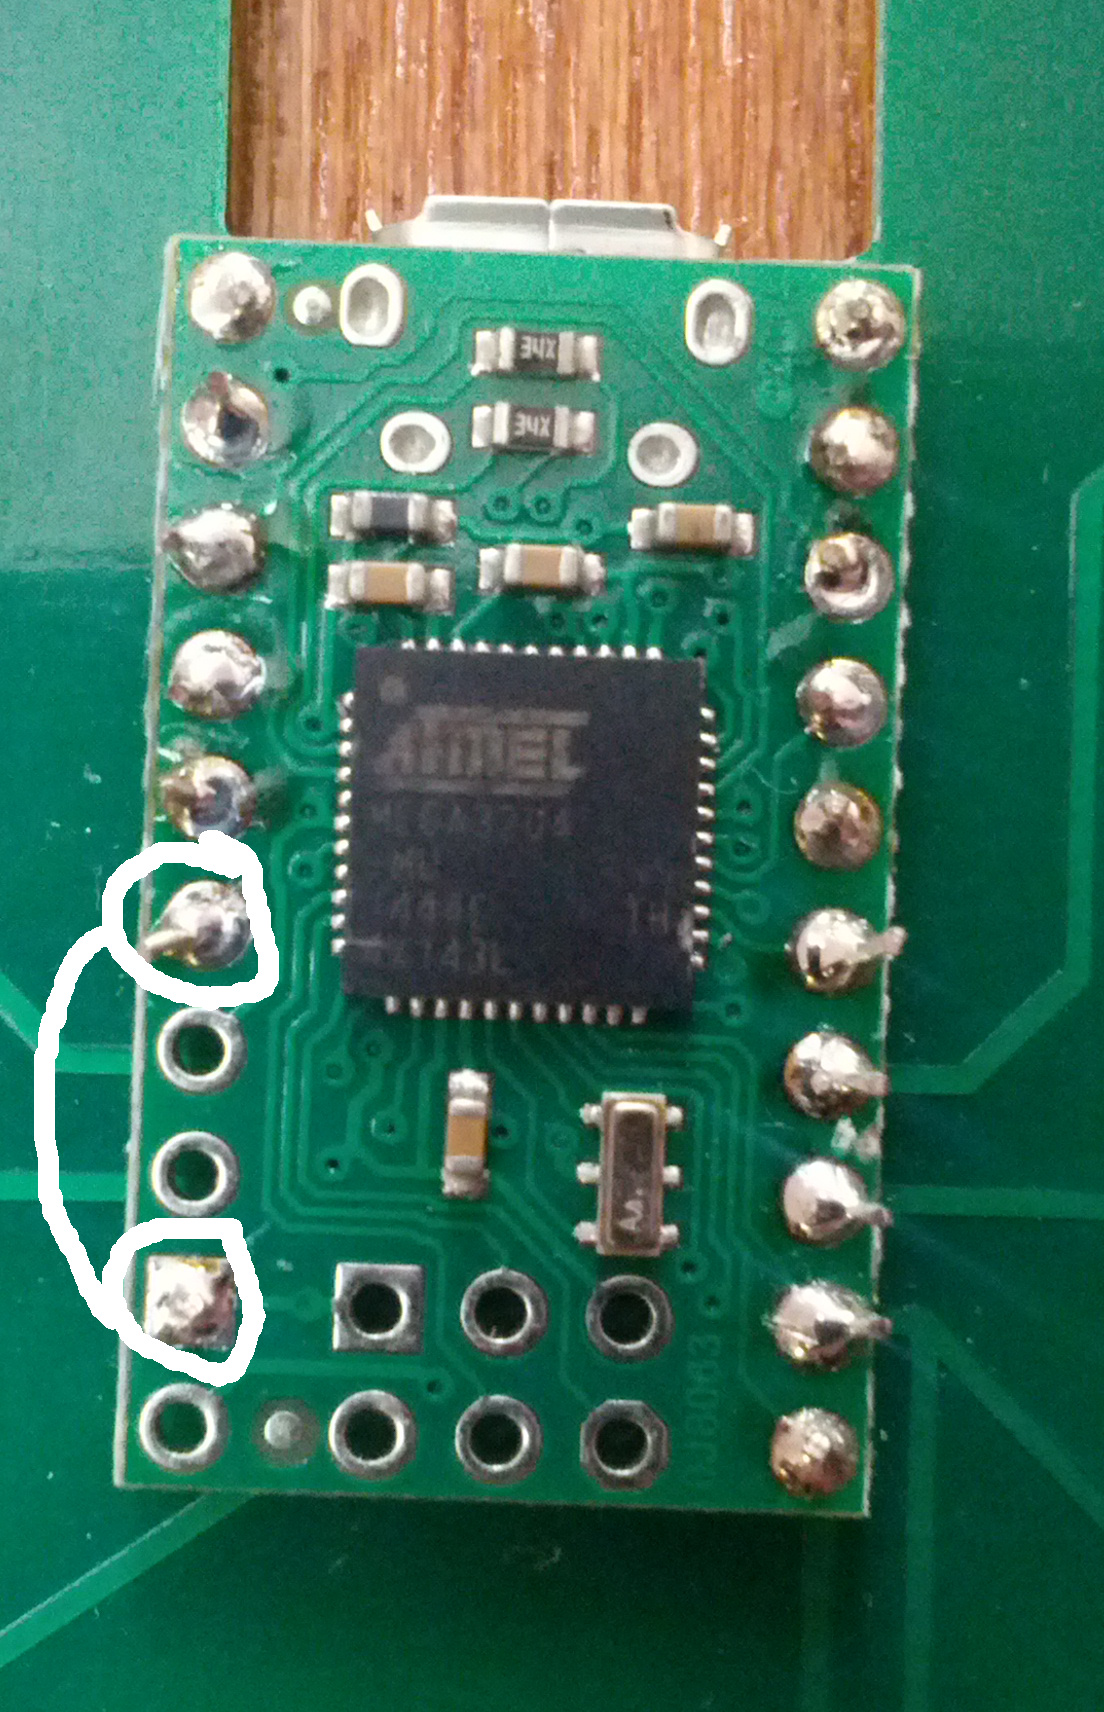
\includegraphics[width=0.8\linewidth]{reset.jpg}
\end{wrapfigure}

Plug in the USB micro cable into the controller, and plug the other
side into your computer. Get a copy of the
firmware \footnote{Available at https://atreus.technomancy.us/tmk} and
its dependencies, \texttt{avrdude} and \texttt{gcc-avr}, linked in the
firmware readme. The first time you upload the firmware, you will have
to use the hardware reset to enter the bootloader: take a diode leg or
wire and touch one end to the reset pin and one end to the ground
pin. (These are circled in the photo.)  Touch them together twice in
under a second and the LED underneath will begin pulsing in a
different pattern from the original blinking. This indicates it has
entered the bootloader for 8 seconds.

\vspace{1em}

While in the bootloader, type \texttt{make upload KEYMAP=qwerty
  USB=[...]}  from the firmware directory\footnote{See the firmware
  readme for instructions about determining the USB argument and
  customizing the layout.}. The firmware should be uploaded, and it
will start functioning as a keyboard once switches are connected. Next
time you upload, you can use the reset key instead of touching the
pins together.

\vspace{1em}

If you only want to use the default layout and don't want to bother
with installing everything, the firmware readme also describes simpler
steps for installing a pre-compiled firmware.

\section{Switches}

Next take four switches and place each switch in a corner of the
switch plate. (The case layer with all the holes in it.) The switches
should be oriented so that the side with pins is to the ``north'' of
the board so they will fit into the holes in the circuit board. Put
the switch plate face-down on the table with the pins sticking
up.

\vspace{1em}

Carefully fit the circuit board over the protruding pins with the
labeled side down. Solder those corners to hold the circuit board and
the switch plate together. The switches should be flush with the
PCB. Take care that the switch pins are straight when you insert them;
pushing in a switch with a pin that's a bit bent will bend it flat and
prevent it from poking through the circuit board.

\vspace{1em}
\noindent\makebox[\textwidth]{%
  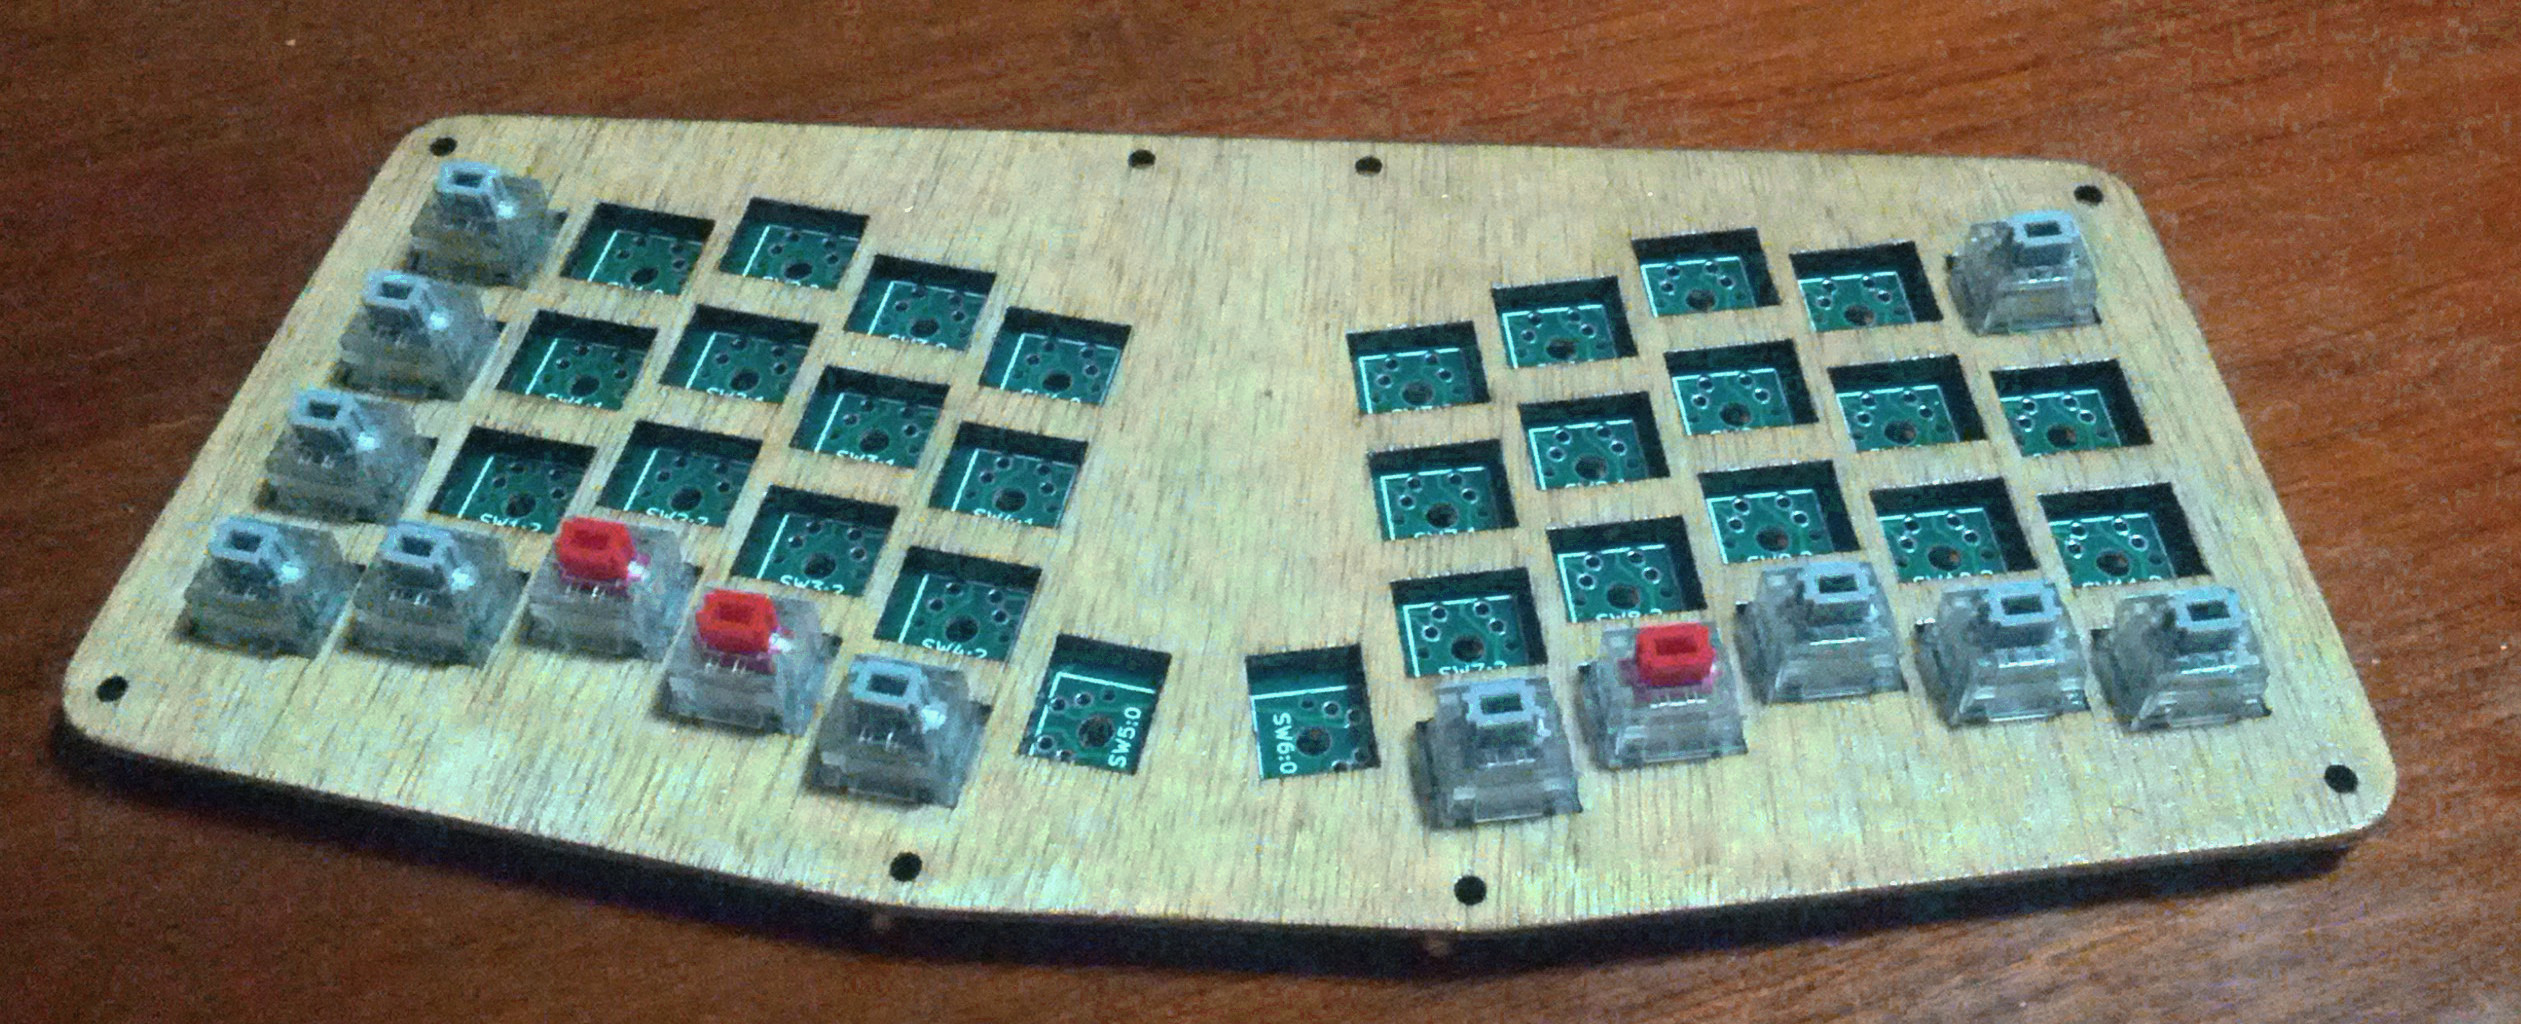
\includegraphics[width=0.7\linewidth]{some-switches.jpg}}
\vspace{1em}

Next fill in the rest of the bottom row (SW1:3 through SW10:3) and the
leftmost column (SW0:1 and SW0:2). If your kit has red linear switches
which do not have any tactile bump, you can choose to use these for
the modifier keys (shift, ctrl, alt, etc) or to leave the modifiers as
normal tactile or clicky keys. Since modifier keys are held down, they
do not benefit from tactility like normal keys do, so some people find
they prefer linear keys there, but this is a matter of personal
taste. The modifiers on the bottom row are SW2:3, SW3:3, and SW8:3.
Place normal switches (usually grey or white) here if you want the
modifiers to feel like the other keys, and red ones if not.

\vspace{1em}

Solder the left and right pins of each of the switches you've placed so
far, and then plug it in to test them to ensure that each row and column is
connected back up to the controller correctly. Once you've confirmed
this, solder the rest of the switches, but leave the middle two
sideways ones for last.

\vspace{1em}
\noindent\makebox[\textwidth]{%
  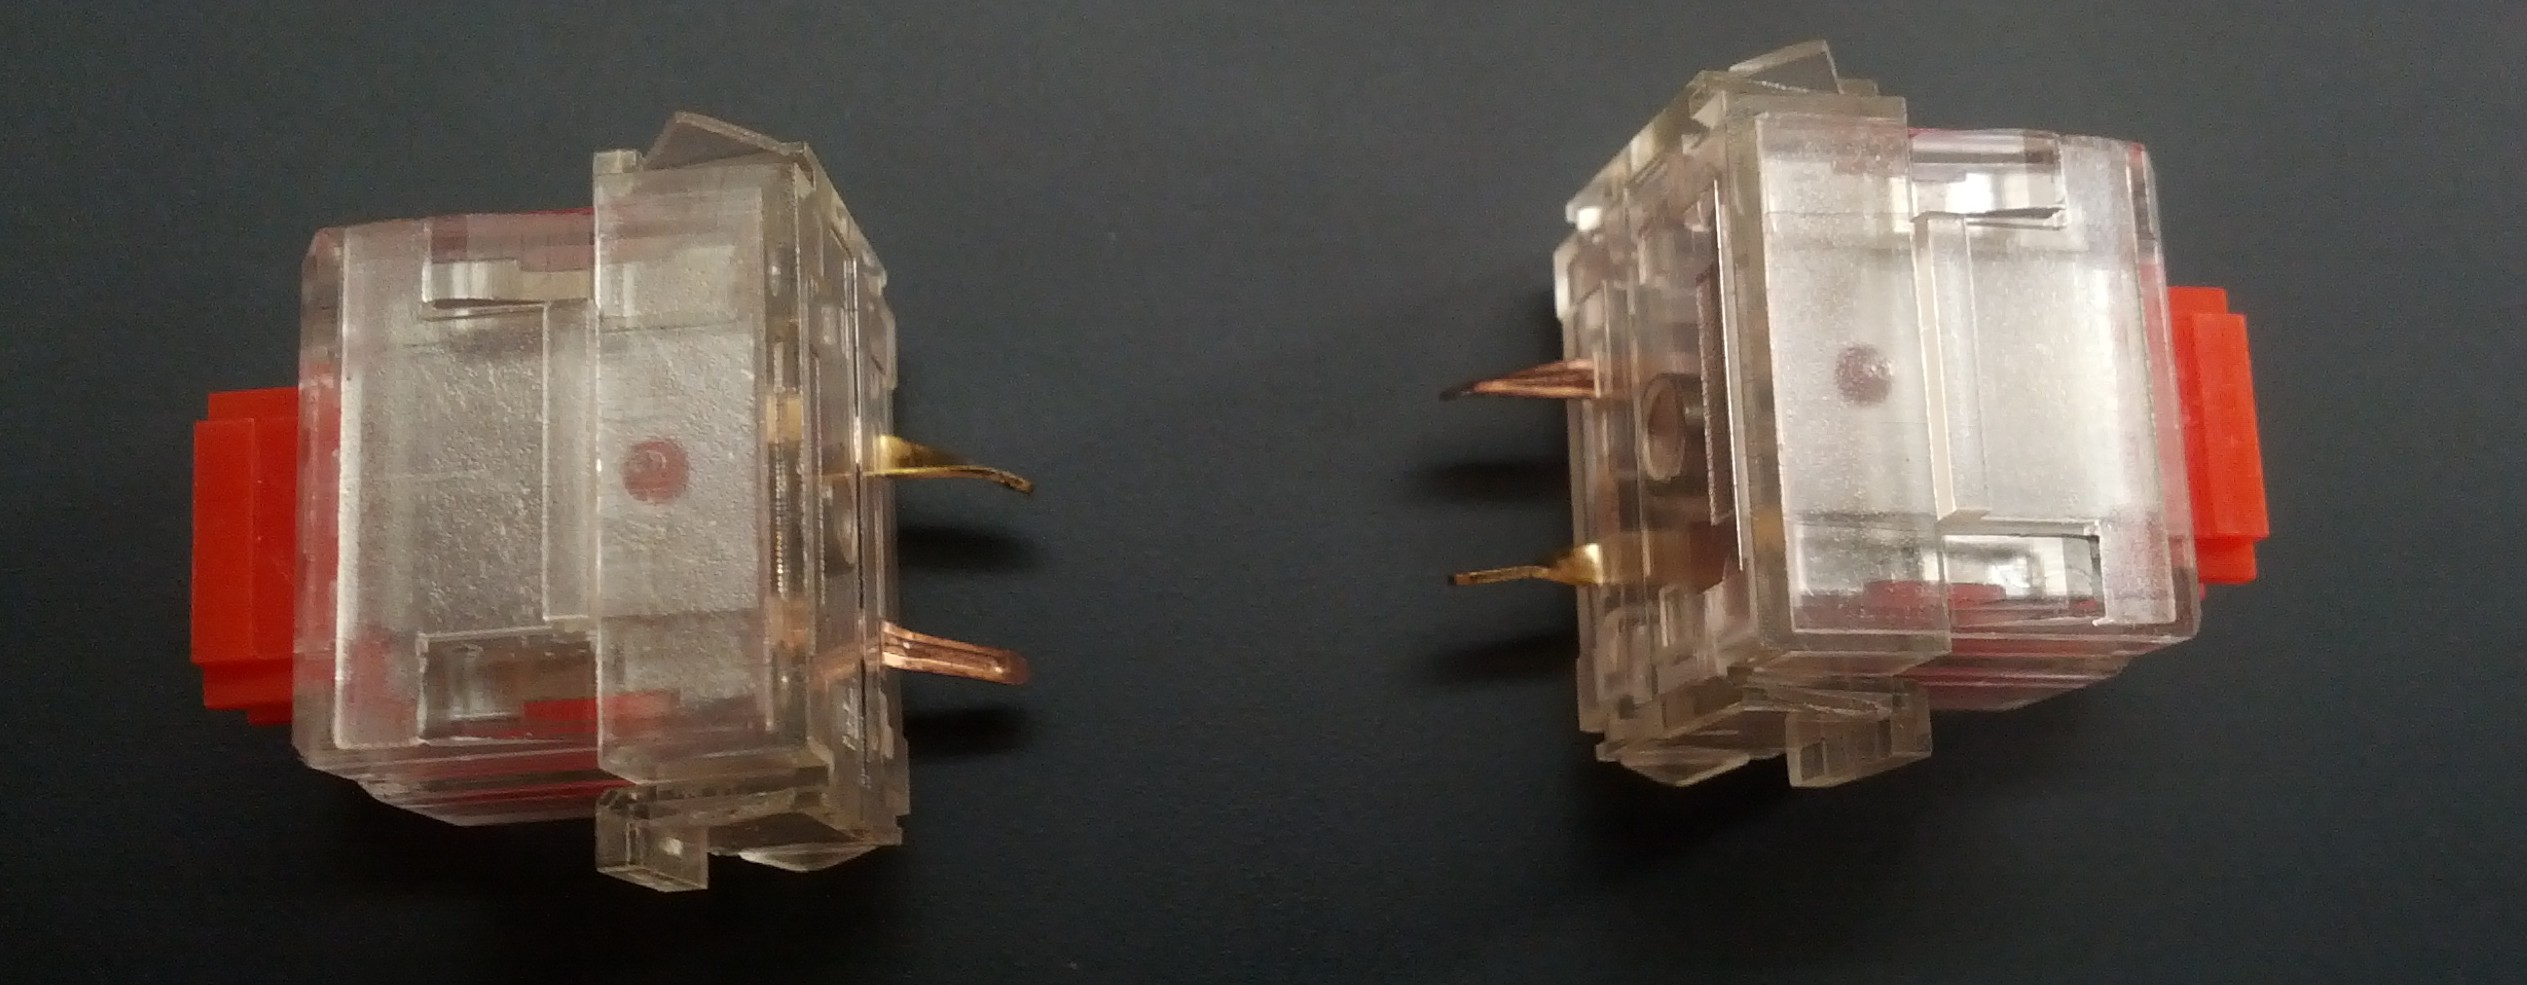
\includegraphics[width=0.8\linewidth]{center-switches.jpg}}
\vspace{1em}

\vspace{1em}

%% The main (non-rotated) switches on Matias kits have their pins
%% positioned a bit lower on the switch than Cherry pins; this shifts
%% the whole PCB a bit further down from where it would be on Cherry kits.

%% The holes for the rotated switches are oriented according to their
%% position on Cherry boards because Cherry switches cannot have their
%% pins twisted; they have a plastic post that helps mount it on the
%% PCB, but moving the middle holes down into the Matias-friendly
%% position would make it completely incompatible with Cherry, while
%% leaving it in the Cherry-friendly position simply makes it slightly
%% inconvenient for Matias kits.

Connecting the center two rotated thumb keys (SW5:0 and SW6:0) in kits
with Matias switches requires a little bit of tweaking. (Cherry
switches do not need this step.) The holes for the pins are not
aligned quite under where the pins protrude. A little twisting will
allow them to go in nicely. Note that the two switches must be twisted
in opposite directions since they are oriented facing away from each
other. You can use pliers or even just your wire cutters to twist
them.

\section{Wrapping Up}

If there's a misbehaving switch, it's often caused by a cold
joint. Reflow the solder on both contacts of the switch and the diode
first; if that doesn't fix it, it may be the connection to the
controller. You can follow the traces for the rows back to the middle,
but the columns on the back of the board are obscured when the
keyboard is assembled; you can see them in this PCB
diagram\footnote{https://atreus.technomancy.us/pcb}.
Re-melting the controller's solder joint for the affected row or
column is usually enough to get it working, but in some cases you may
need to reach under to get the joint that connects it to the PCB.

\vspace{1em}

If there is room between the head of the USB cable and the place where
the cable leaves the case, consider adding strain relief by wrapping
the cable with electrical tape at the point just below where it leaves
the case. This will make it so pulling on the cable does not dislodge
it from the controller.

\vspace{1em}

After the switches are all in and tested, place the keycaps. They can
take a fair bit of pressure to go on, so support the underside of the
board while pushing them on. The larger keycaps go on the middle thumb
keys.

\vspace{1em}

All that's left is to do is close the case by placing the switch plate
on top of the spacer and bottom plate, placing the top plate on it,
and screwing it together with the nuts facing up. If the controller
was not attached close enough to the circuit board, it may be
necessary to sand down the USB connector in order to close the
case. Before you place the rubber feet on the bottom plate near the
corners, consider giving the outer case another coat or two of wax and
allowing it to dry. If the rubber feet don't stay on with the provided
adhesive, white glue may be needed to secure them.

\vspace{1em}

Congratulations. Enjoy your new keyboard. It will take a
considerable adjustment period to get used to it, but it should result
in much more comfortable and effective typing. Also remember that
you're encouraged to customize the layout to make it truly your
own. Happy typing!

%% \noindent\makebox[\textwidth]{%
%% 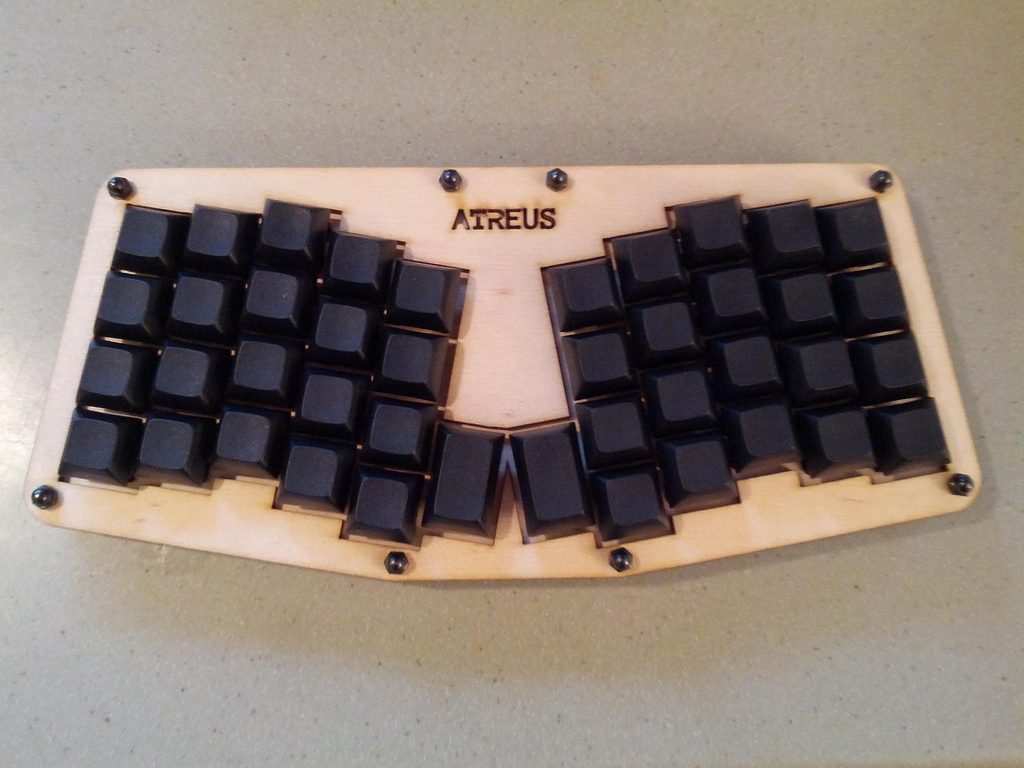
\includegraphics[width=\linewidth]{finished.jpg}}

\end{document}
